\chapter{iview: WebGL visualizer for protein-ligand complex}

\section{Abstract}

Visualization of protein-ligand complex plays an important role in elaborating protein-ligand interactions and aiding novel drug design. Most existing web visualizers either rely on slow software rendering, or lack the support of macromolecular surface construction. The useful feature of virtual reality is also unavailable.

We have developed iview, an easy-to-use interactive WebGL visualizer for protein-ligand complex. It exploits hardware acceleration rather than software rendering, and supports four surface representations including Van der Waals surface, solvent excluded surface, solvent accessible surface and molecular surface. It features four special effects in virtual reality settings, namely anaglyph, parallax barrier, oculus rift and stereo, leading to visually appealing identification of intermolecular interactions. Moreover, based on the feature-complete version of iview, we have also developed a concise and tailor-made version specifically for our istar::idock to aid online protein-ligand docking service. This demonstrates the excellent portability of iview.

Using innovative 3D techniques, we provide a user friendly visualizer that is not intended to compete with professional visualizers, but to permit easy accessibility and platform independence. To the best of our knowledge, iview is the only web visualizer that utilizes GPU hardware acceleration and supports three unique features: protein surface construction, virtual reality effects, and PDBQT format input. iview is freely available at http://istar.cse.cuhk.edu.hk/iview.

This was a collaborative project with Takanori Nakane from Graduate School of Medicine, Kyoto University, Japan. It was published in \textit{BMC Bioinformatics} on 25 February 2014 \citep{1366}. Notably, this article has been tagged ``Highly accessed" by the journal, indicating that it may be of broad interest in the community.

\section{Introduction}

Protein-ligand visualization serves an important role in elaborating intermolecular interactions and aiding novel drug design. To date, dozens of visualization tools already exist. VMD \citep{1220}, PyMOL (http://www.pymol.org) and Chimera \citep{1219} are quite well-known and highly cited. They can interpret multiple file formats, generate multiple representations, and provide precise control. BINANA \citep{1413} characterizes ligand-binding and outputs a state file compatible for display in VMD \citep{1220}. AutoDockTools4 \citep{596} provides native support for the PDBQT file format, which is widely used in various protein-ligand docking software such as AutoDock \citep{596}, AutoDock Vina \citep{595}, QuickVina \citep{1193} and our idock \citep{1153}. We also developed our own tool \citep{1265} to visualize structures in virtual reality settings and employ fragment-based \textit{de novo} ligand design strategy for use in interactive drug design. PoseView \citep{748} and LigPlot+ \citep{951}, on the other hand, plot 2D diagrams of protein-ligand interactions from 3D coordinates.

In addition to the above standalone visualizers, there are web-based visualizers using either Java applet, Adobe Flash, or HTML5 canvas. Jmol (http://www.jmol.org), an open source Java viewer for chemical structures in 3D, has been deployed worldwide and recognized as the \textit{de facto} molecular viewer on the web. GIANT \citep{1359}, a Jmol derivative, supports analyzing protein-ligand interactions on the basis of patterns of atomic contacts obtained from the statistical analyses of 3D structures. Unfortunately, Java is being disabled on more and more systems due to security concerns. Hence Java-free visualizers are highly desired. JSmol \citep{1314}, a JavaScript-only version of Jmol, includes the full implementation of the entire set of Jmol functionalities. Although Jmol and JSmol support a large set of advanced features such as scripting, they rely on software rendering which is slow on large display areas and thus prevents detailed inspection of the structure. In contrast, WebGL visualizers benefit from GPU hardware acceleration. For instance, ChemDoodle Web Components (http://web.chemdoodle.com), a pure JavaScript chemical graphics and cheminformatics library, presents 2D and 3D graphics and animations for chemical structures, reactions and spectra, but it lacks protein surface construction. GLmol (http://webglmol.sourceforge.jp), a molecular viewer on WebGL/JavaScript using the three.js library, supports multiple file formats and representations, and features an experimental version of surface construction based on the EDTSurf algorithm \citep{1297,1350}, an experimental version of atomic labeling and click-to-identifying, and an experimental version of electron density map visualization by isomesh or volume rendering. Another WebGL technology \citep{1262} also supports rendering molecular surface using the SpiderGL library \citep{1320}. However, none of these WebGL visualizers except JSmol support virtual reality effects.

Surface representation is a convenient way to visualize protein-ligand interactions. Nevertheless, macromolecular surface calculation is computationally and memory intensive. Furthermore, the calculated mesh is fairly complex, often exceeding 500,000 polygons. Therefore its implementation in JavaScript/WebGL has been considered very difficult. Most existing web visualizers either rely on slow software rendering, or lack virtual reality support. Moreover, the important feature of protein surface construction is usually unavailable, and the support for PDBQT format is not implemented.

To address the above obstacles, we have developed iview, an interactive WebGL visualizer of protein-ligand complex, featuring four special effects in virtual reality settings and four macromolecular surface representations. Furthermore, we show that iview can be easily modified to adapt to different applications. As an application example, we have refactored the feature-rich version of iview and derived a tailor-made version specifically for visualizing istar::idock input data and output results of user-submitted jobs.

\section{Methods}

iview is refactored from GLmol 0.47 and uses three.js as its primary 3D engine with anti-aliasing support. It is based on WebGL canvas and can be easily integrated into existing HTML5 web pages to display molecular models without requiring Java or browser plugins. It loads a protein-ligand structure from the PDB (Protein Data Bank) \citep{1357} as its data source via a RESTful interface. It renders four standard representations of primary structure, namely line, stick, ball \& stick and sphere, and five standard representations of secondary structure, namely ribbon, strand, cylinder \& plate, C alpha trace and B factor tube. It colors the structure by either atom spectrum, protein chain, protein secondary structure, B factor, residue name, residue polarity, or atom type, by setting the vertex colors of the geometry object of the corresponding representation. It supports user interactions including rotation, translation, zooming and slab with mouse or hand touch manipulation. It provides both perspective and orthographic cameras, and anaglyph, parallax barrier, oculus rift and stereo effects from three.js examples for use in a virtual reality environment. It supports exporting the WebGL canvas to PNG (Portable Network Graphic) which can be subsequently embedded in a document.

We ported EDTSurf \citep{1297,1350}, an fast algorithm to generating triangulated macromolecular surfaces by Euclidean distance transform, to JavaScript and integrated it into iview to construct and render in real time four representations of protein surface, namely Van der Waals surface, solvent excluded surface, solvent accessible surface and molecular surface, with opacity and wireframe adjustable by users. Note that molecular surface is in fact solvent excluded surface, but EDTSurf uses different ways to derive them. So we provide them both as two different surface representations in iview. Although the JavaScript implementation of the EDTSurf algorithm typically consumes a few seconds and 500MB to 700MB memory for computation, it is sufficiently efficient for practical applications. To limit CPU and memory usage, the calculation grid size is restricted to 180 x 180 x 180.

\section{Results}

Table \ref{iview:features} lists the full features of iview.

\begin{table}
\caption{iview features.}
\label{iview:features}
\begin{tabular}{ll}
\hline
                 Category & Features\\
\hline
        File format input & PDB\\
                          & PDBQT\\
\hline
                   Camera & perspective\\
                          & orthographic\\
\hline
               Background & black\\
                          & grey\\
                          & white\\
\hline
       Structure coloring & atom spectrum\\
                          & protein chain\\
                          & protein secondary structure\\
                          & B factor\\
                          & residue name\\
                          & residue polarity\\
                          & atom type\\
\hline
        Primary structure & line\\
                          & stick\\
                          & ball \& stick\\
                          & sphere\\
                          & dot\\
\hline
      Secondary structure & ribbon\\
                          & strand\\
                          & cylinder \& plate\\
                          & C alpha trace\\
                          & B factor tube\\
\hline
          Protein surface & Van der Waals surface\\
                          & solvent excluded surface\\
                          & solvent accessible surface\\
                          & molecular surface\\
\hline
 Proteins surface opacity & 1.0, 0.9, 0.8, 0.7, 0.6, 0.5\\
\hline
Protein surface wireframe & yes, no\\
\hline
Atom and residue labeling & yes, no\\
\hline
   Virtual reality effect & anaglyph\\
                          & parallax barrier\\
                          & oculus rift\\
                          & stereo\\
\hline
      Canvas manipulation & mouse\\
                          & hand touch\\
\hline
        Manipulation mode & rotation\\
                          & translation\\
                          & zooming\\
                          & slab\\
\hline
            Canvas export & png\\
\hline
\end{tabular}
\end{table}

We take as an example the CCR5 chemokine receptor-HIV entry inhibitor maraviroc complex (PDB: 4MBS) \citep{1348}. Figures in this section can be reproduced at http://istar.cse.cuhk.edu.hk/iview/?4MBS. Figure \ref{iview:ribbon} shows the human CCR5 secondary structure rendered as ribbon, and the marketed HIV drug maraviroc rendered as sphere.

\begin{figure}
\begin{center}
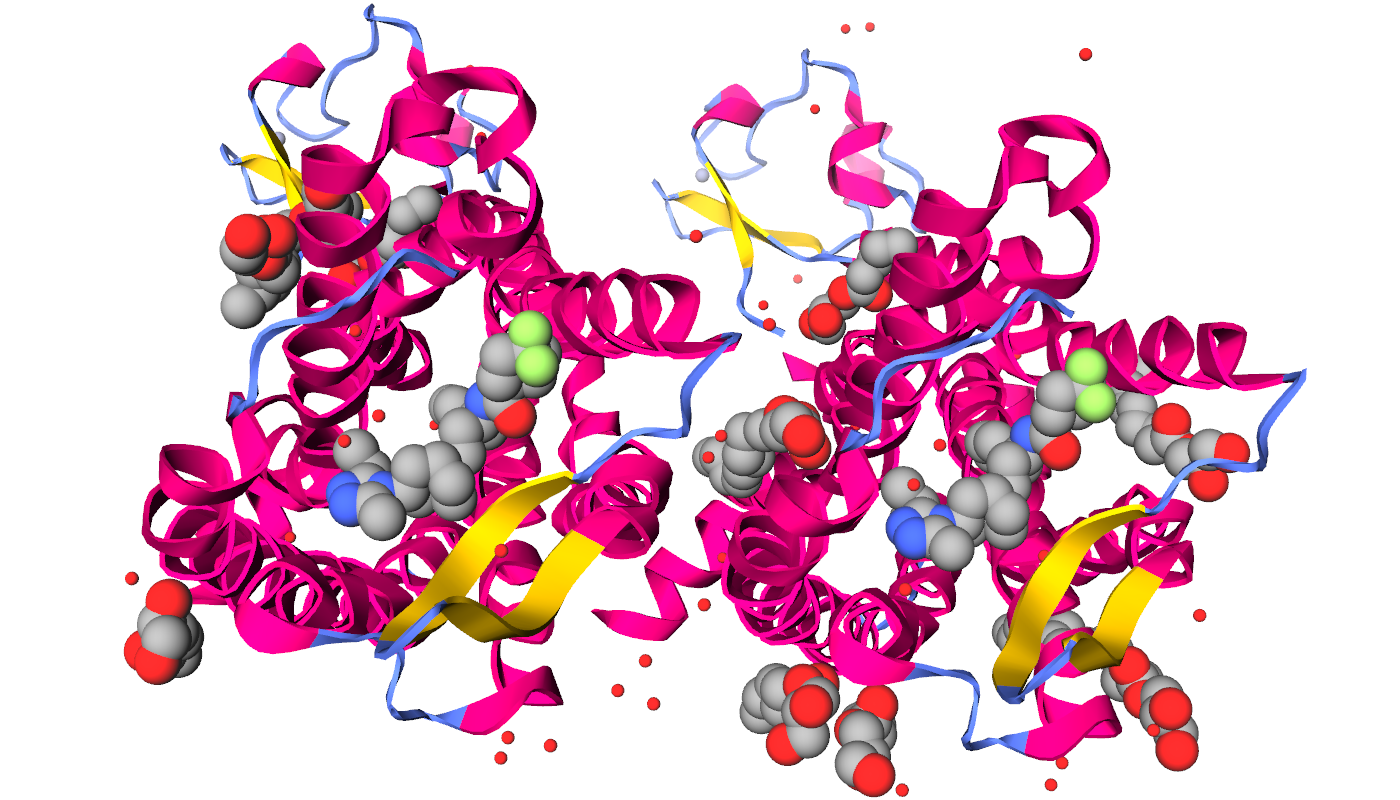
\includegraphics[width=\linewidth]{../iview/ribbon.png}
\end{center}
\caption{iview rendering of the CCR5 chemokine receptor-HIV entry inhibitor maraviroc complex.}
\label{iview:ribbon}
\end{figure}

Figure \ref{iview:anaglyph} shows the anaglyph effect in a virtual reality environment. The anaglyph effect encodes each eye's image using filters of chromatically opposite colors to achieve stereoscopic 3D effect. When users wear a spectacle with special filters on both sides, each of the two differently filtered colored images reaches one eye, revealing an integrated stereoscopic image. The disparity between two superimposed molecules creates a perception of depth, leading to visually more appealing identification of intermolecular interactions.
 
\begin{figure}
\begin{center}
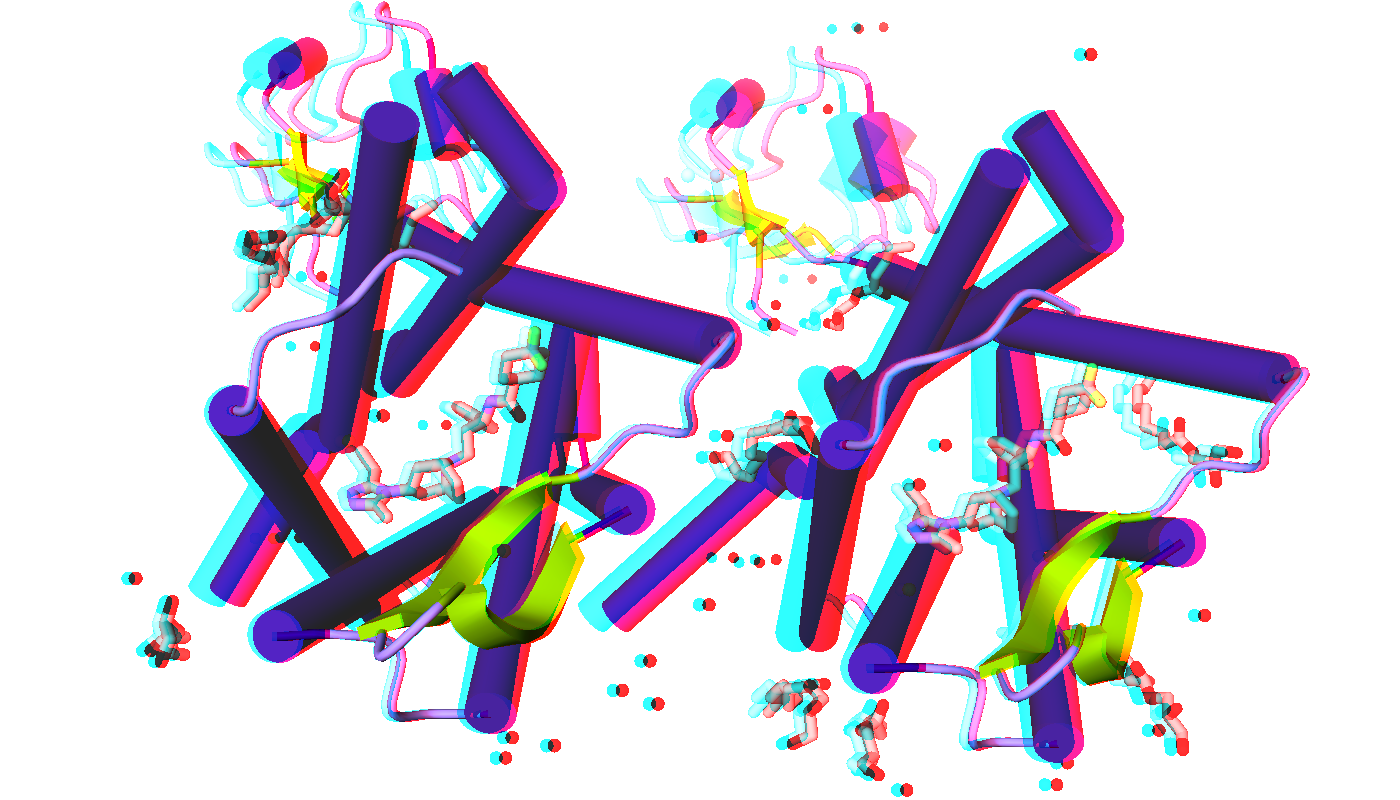
\includegraphics[width=\linewidth]{../iview/anaglyph.png}
\end{center}
\caption{iview rendering of the CCR5 chemokine receptor-HIV entry inhibitor maraviroc complex, with anaglyph effect enabled.}
\label{iview:anaglyph}
\end{figure}

Figures \ref{iview:parallaxbarrier} illustrates the parallax barrier effect. A parallax barrier is a device placed in front of a LCD (Liquid Crystal Display) to permit a stereoscopic or multiscopic image without 3D glasses. The device is composed of a layer of material with precision slits, enabling each eye to see a different set of pixels and thus creating a sense of depth through parallax.

\begin{figure}
\begin{center}
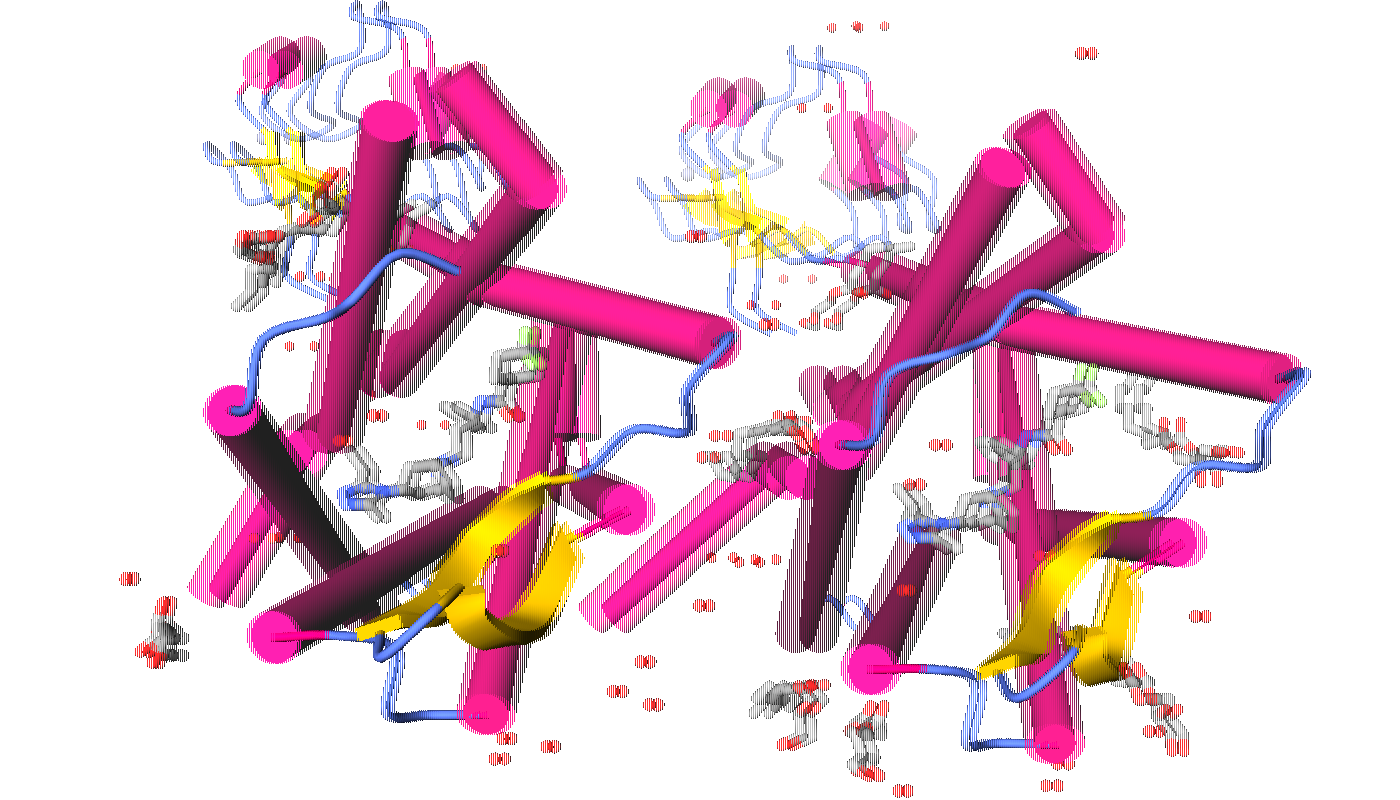
\includegraphics[width=\linewidth]{../iview/parallaxbarrier.png}
\end{center}
\caption{iview rendering of the CCR5 chemokine receptor-HIV entry inhibitor maraviroc complex, with parallax barrier effect enabled.}
\label{iview:parallaxbarrier}
\end{figure}

Figure \ref{iview:oculusrift} illustrates the oculus rift effect. The cculus rift is a virtual reality head-mounted device, which features a high-speed inertial measurement unit and a LCD display, visible via dual lenses positioned over the eyes to provide a 90 degrees horizontal and 110 degrees vertical stereoscopic 3D perspective.

\begin{figure}
\begin{center}
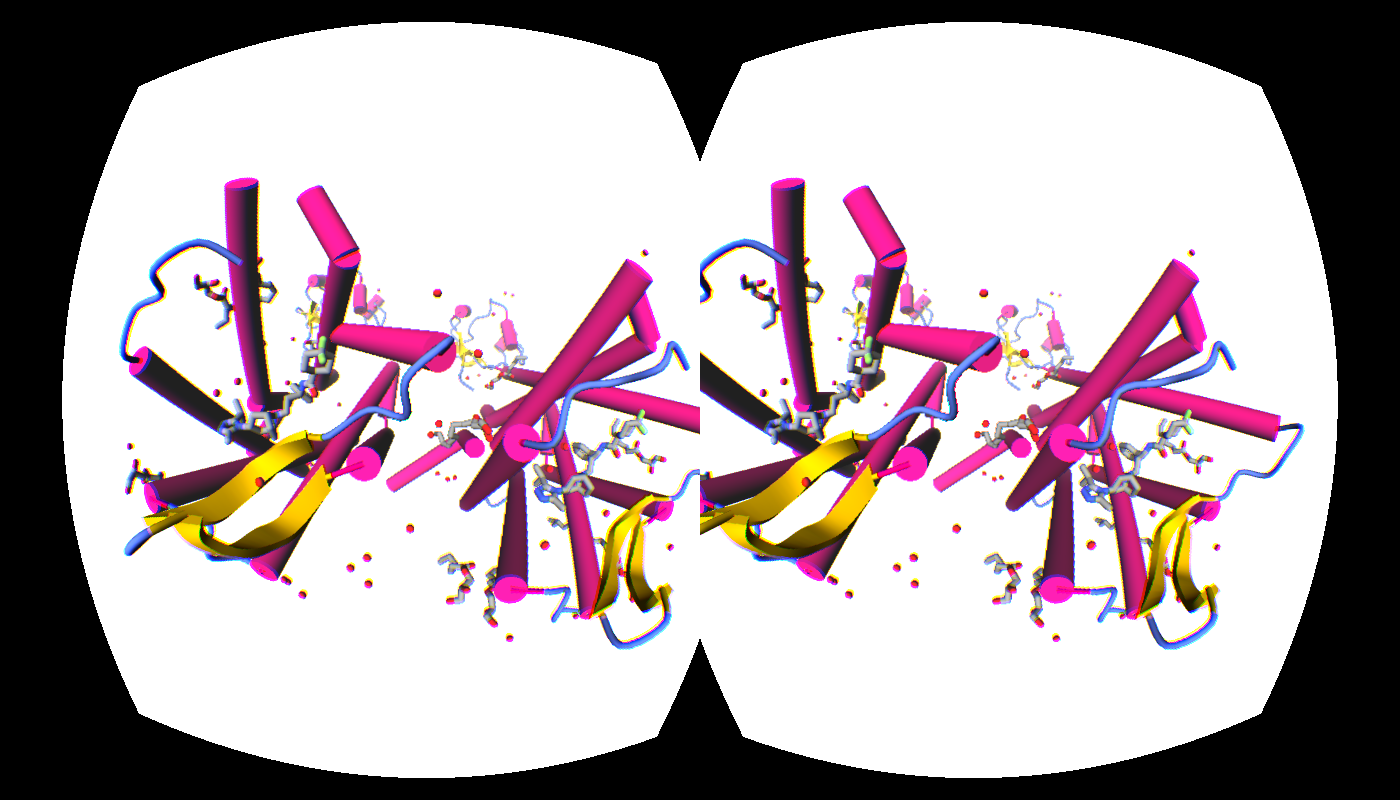
\includegraphics[width=\linewidth]{../iview/oculusrift.png}
\end{center}
\caption{iview rendering of the CCR5 chemokine receptor-HIV entry inhibitor maraviroc complex, with oculus rift effect enabled.}
\label{iview:oculusrift}
\end{figure}

Figure \ref{iview:surface} shows the protein surface generated by our JavaScript implementation of the EDTSurf algorithm \citep{1297,1350}. The human CCR5 is rendered as molecular surface colored by chain. The marketed HIV drug maraviroc is rendered as stick colored by chain. It can be clearly seen that the asymmetric unit is composed of two complexes, and the CCR5 forms a deep allosteric cavity where maraviroc is buried.

\begin{figure}
\begin{center}
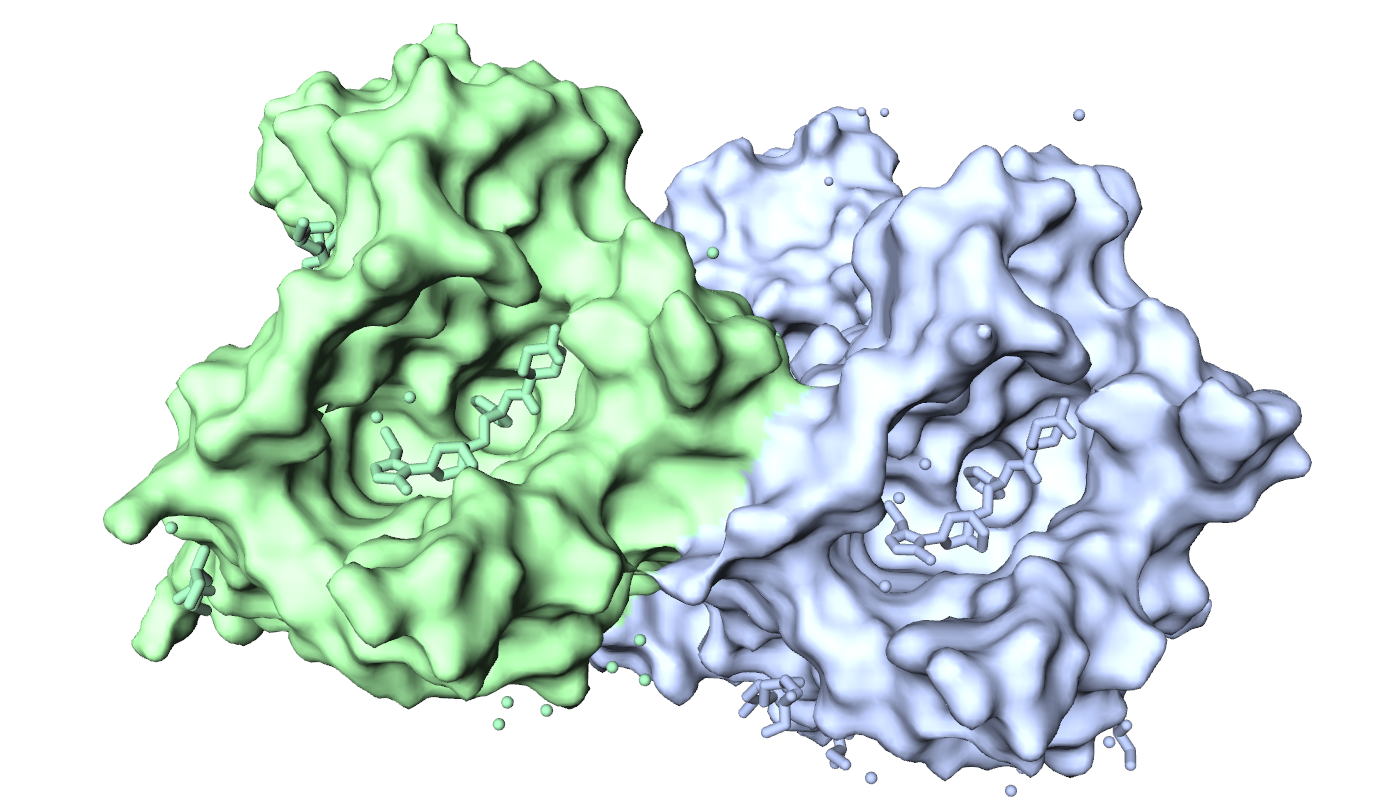
\includegraphics[width=\linewidth]{../iview/surface.png}
\end{center}
\caption{iview rendering of the CCR5 chemokine receptor-HIV entry inhibitor maraviroc complex, with protein molecular surface enabled.}
\label{iview:surface}
\end{figure}

\section{Application}

We emphasize portability and usability, and illustrate that iview can be easily modified to suit one's particular application, given that iview is free and open source under a permissive license. We take protein-ligand docking as an example. Based on the feature-rich version of iview, our tailor-made version specifically for istar::idock cleans up many dispensable functions, enabling a very neat interface. It only retains the rendering of primary structure of protein and ligand, and the construction of protein surface. Most importantly, it implements new features especially for protein-ligand docking purpose. Figure \ref{iview:idock} shows this application-specific version and can be reproduced at http://istar.cse.cuhk.edu.hk/idock/iview/?525a0abab0717fe31a000001.

In the input phase of a docking job, it merely requires a PDB file, which can be obtained either from the PDB database \citep{1357} or via homology modeling, and then constructs the protein surface asynchronously in a separate web worker to keep the web page responsive. It automatically detects a binding site from the largest co-crystallized ligand first by finding the smallest cubic box that covers the entire ligand and then by extending the box by 50\% in all the three dimensions in order to reserve space for conformational sampling. In case of non-existence of co-crystallized ligand, the binding site is defaulted to the geometric center of the protein. The binding site is visually depicted in the form of a cubic box whose center and size can be manually adjusted by users in real time.

In the output phase of a docking job, it displays the user-supplied cubic box for users to confirm that the predicted ligand conformations do fall inside the desired binding site. Other than PDB format, its parsers are capable of parsing a protein and multiple top hit ligands in PDBQT format used by idock. It displays the top hit ligand IDs in a horizontally scrollable row and provides a straightforward way to switch ligands easily through a button group. It has built-in support for putative intermolecular hydrogen bond detection by finding hydrogen bond donors and acceptors from protein and ligand and setting the distance threshold to 3.5\AA. It automatically annotates important atoms, like those involving in intermolecular hydrogen bonds, by placing labels next to the corresponding atoms in the canvas. It lists the docking result files, predicted free energy and binding affinity values, molecular properties, SMILES representation, compound suppliers and annotations, and putative hydrogen bond positions and their lengths, in order to give users a quick overview of the top hit ligands and assist them in making decisions of which compounds to purchase for subsequent wet-lab experiments.

\begin{figure}
\begin{center}
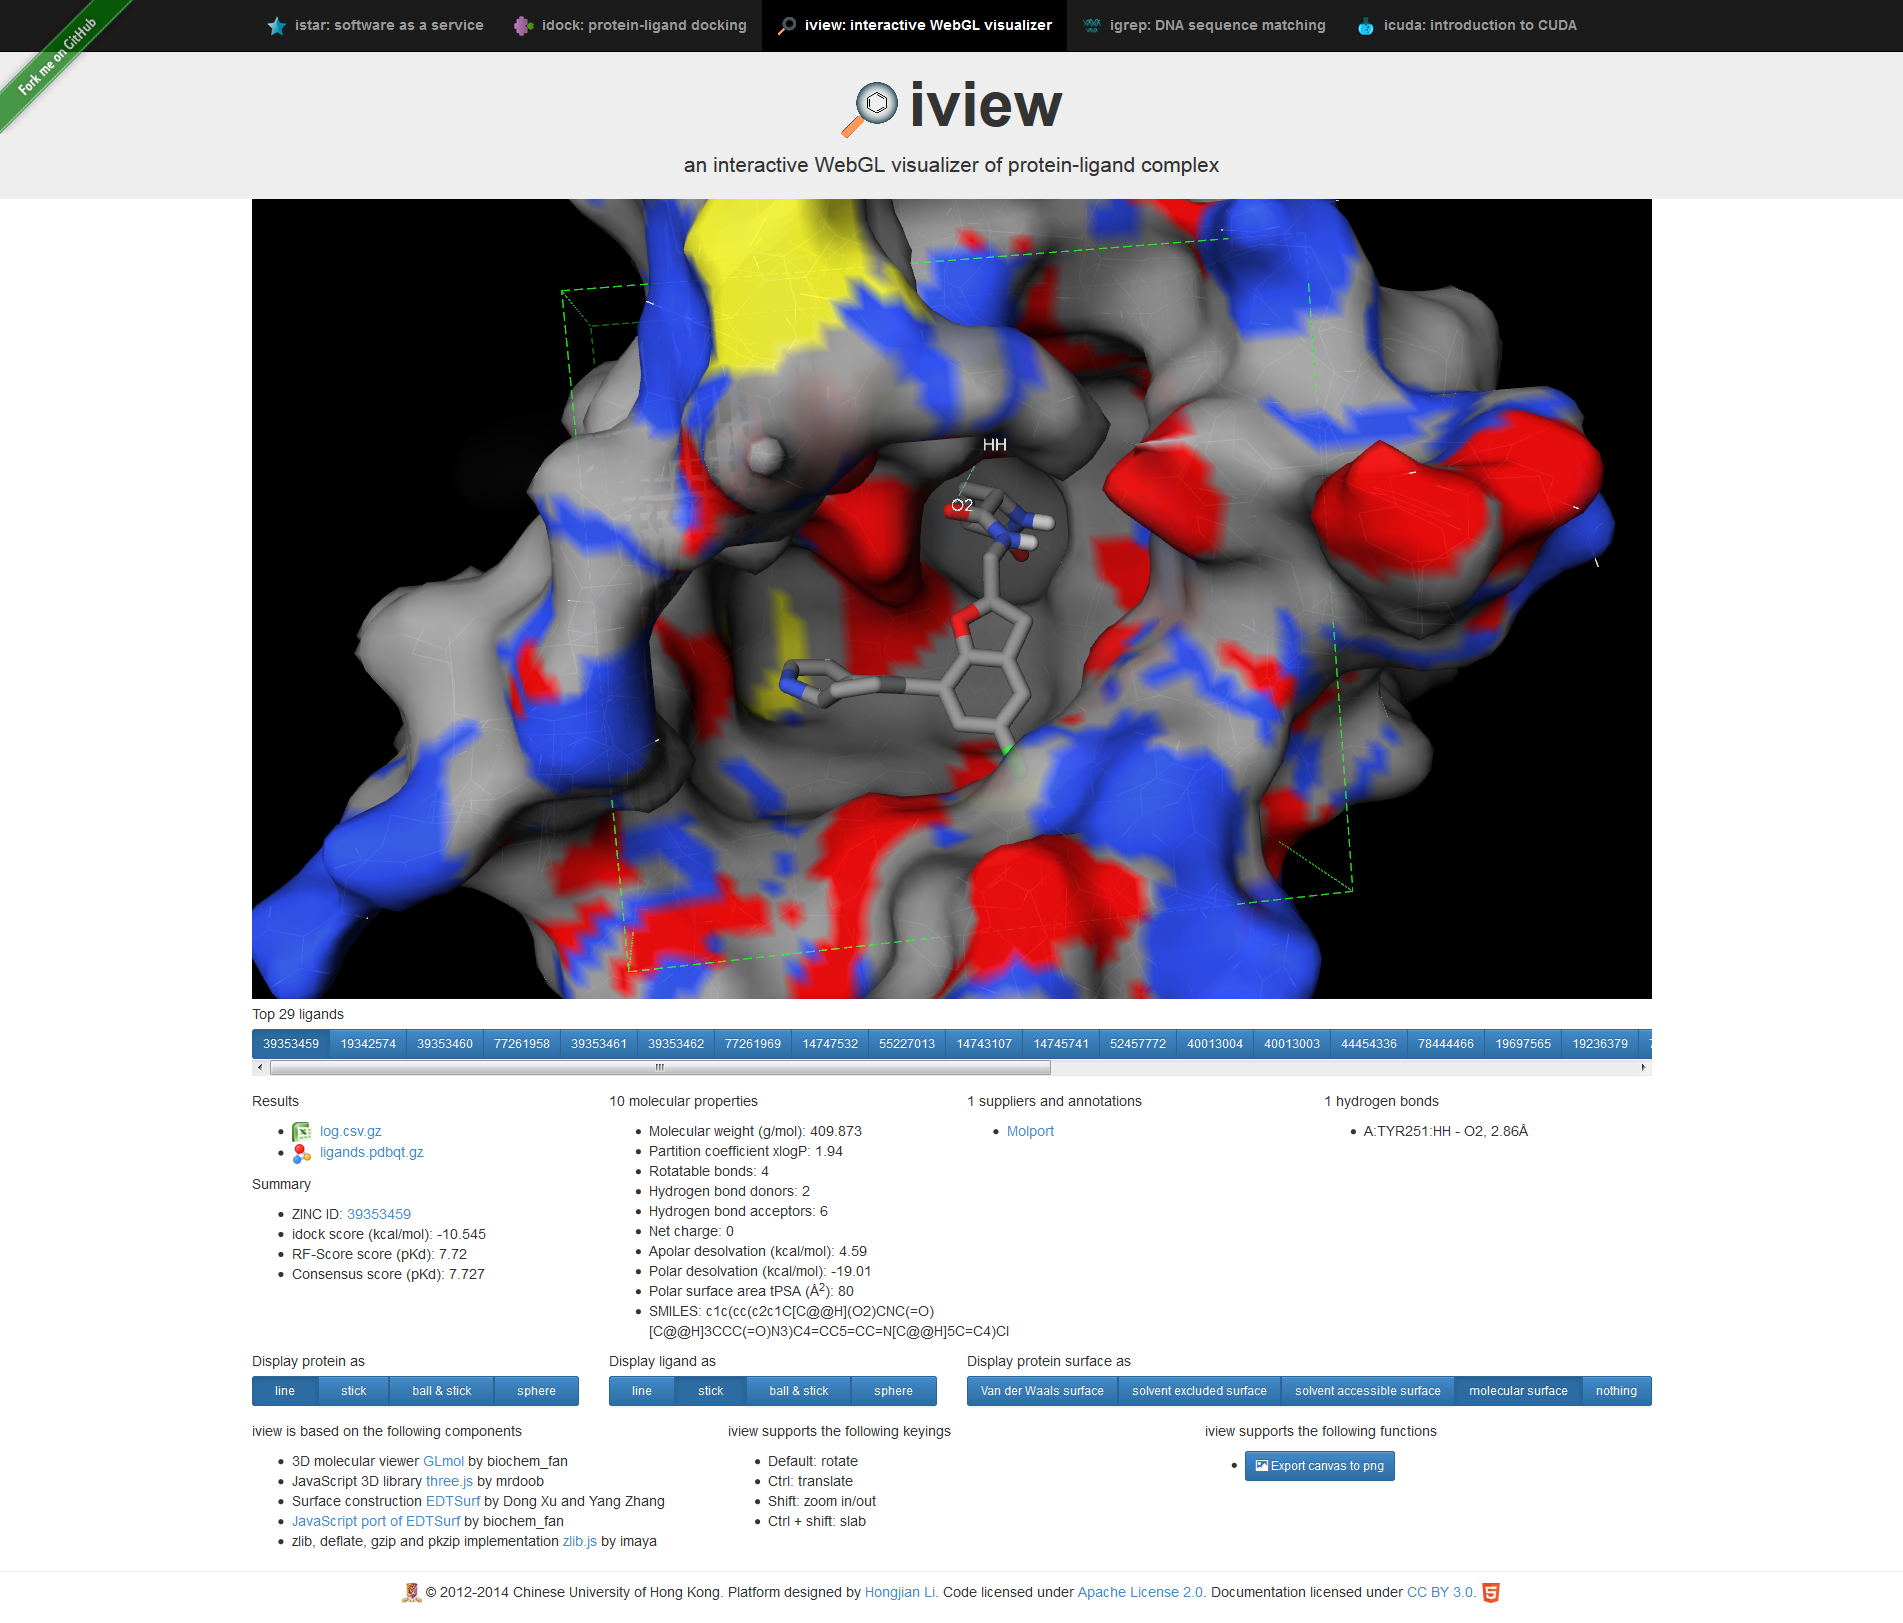
\includegraphics[width=\linewidth]{../iview/idock.png}
\end{center}
\caption{Tailor-made version of iview specifically for visualizing istar::idock results of user-submitted jobs.}
\label{iview:idock}
\end{figure}

\section{Discussion}

We developed iview with the purpose to simplify and promote the use of istar::idock. At first we tried ChemDoodle Web Components, but it had strong dependency on its server side components, whose source code we had no access to. Later we turned to GLmol, although which has been discontinued since 29 August 2012, was quite an exciting project because it gracefully built its geometric modeling and relevant functions on top of the three.js foundation, and thus greatly reduced the programming difficulty.

Based on GLmol, iview has fixed many bugs and meanwhile introduced new features. Their differences are as follows. iview supports four virtual reality effects, which GLmol lacks. iview allows users to choose a surface opacity between 1.0 and 0.5 so that users can inspect both protein surface and internal structures at the same time. iview can parse alternate atoms and reconstruct their covalent bonds, but GLmol simply ignores them. iview can identify metal ions and highlight their bonds by dashed lines. GLmol does not distinguish metal ions and displays their bonds by ordinary lines. iview supports as many as 100 atom types, from H to Fm, i.e. the first 100 atoms in the periodic table. GLmol can only recognize about 16 common atoms.

Furthermore, the tailor-made version specifically for protein-ligand docking also supports the following features: parsing of the PDBQT file format, which is widely used in the most cited AutoDock series and our idock software; automatic protein binding site detection using the position and molecular size of the co-crystallized ligand; automatic detection and display of intermolecular hydrogen bonds; automatic annotation of important atoms, such as those involving in intermolecular hydrogen bonds; asynchronous generation of protein surface by a web worker, making the web page responsive; result file gzip decompression by the zlib.js library; and fast toggling among different representations via in-memory caching.

It is worthwhile to highlight that iview performs all parsing and rendering in the client browser, with no dependency on the server side at all, thus ensuring the data privacy is maintained. This is unlike ChemDoodle Web Components, some of whose functions send data to a dedicated server for processing and wait for retrieval of results.

\section{Conclusions}

We have designed and developed iview to be a simple and straightforward way to visualize protein-ligand complex. It enables non-experts to quickly elucidate protein-ligand interactions in a 3D manner. Furthermore, iview is free and open source, and can be easily integrated into any bioinformatics application that requires interactive protein-ligand visualization. As far as we are aware, iview is the unique web visualizer that simultaneously utilizes GPU hardware acceleration and supports three pragmatic features: macromolecular surface construction, virtual reality effects, and PDBQT format parsing.

\section{Availability}

iview is free and open source under Apache License 2.0. It is written in JavaScript, HTML5 and CSS3, and available at http://istar.cse.cuhk.edu.hk/iview. It is independent of operating systems but requires a browser and a graphics card with WebGL capability. It has been successfully tested in Chrome 30, Firefox 25, Safari 6.1 and Opera 17. Support for IE 11 is experimental because gl\_FrontFacing is unsupported in IE 11. Refer to http://caniuse.com/webgl for compatibility of WebGL support in desktop and mobile browsers.

\section{Future works}

Both BINANA \citep{1413} and GIANT \citep{1359} can characterize protein-ligand interaction patterns. BINANA, for instance, identifies key binding characteristics like hydrophobic contacts, hydrogen bonds, salt bridges, and pi interactions. Integrating these algorithms will make iview even more pragmatic.

%HPC WebGL

\chapterend
